% Architecture figure for the HPEC systems paper: how a heterogeneous forest of
% SR trees maps onto the GPU, and the host-driven batched-LM execution model.
%
% Faithful to the implementation (same sources as lm_algorithm.tex):
%   cusr/kernel/batch_lm_fusedfd.cu  (fd_jacobian_fused_kernel, build_jtj_jtr, solve)
%   cusr/kernel/ad_interp.cuh        (ad_jacobian_kernel)
%   cusr/kernel/lm_core.cuh          (eval/residual/loss kernels, fp64 boundary audit)
%   cusr/kernel/co_lib.cu            (the in-process LM-loop body: host `for it` at L343,
%                                     ad_jacobian L351, build_jtj_jtr L388, co_solve L393,
%                                     per-iter H<->D of lam/delta/loss/status L392-396)
%
% HONESTY NOTE (why panel (b) is NOT one fused mega-launch):
%   The LM loop is a HOST driver. Each iteration issues SEPARATE device launches
%   (BuildJacobian -> Assemble -> SolveDamped -> Eval), and small per-tree state
%   (lambda, delta, loss, status) crosses the H<->D boundary every iteration.
%   The narrow, true "single launch" claim is per-STAGE: one launch covers all M
%   heterogeneous trees (warp-per-tree), instead of M per-tree launches. Drawing
%   the whole solve as one kernel would misrepresent it: the LM loop is multiple per-iter
%   kernel launches + a host-side accept/reject outer loop. The H<->D boundary is structural
%   but only ~2-5% of runtime; the loop is GPU-bound (Jacobian ~60-66%, issue/instruction-
%   bound), NOT host-orchestration-bound (refuted — see OPTIMIZATION_BACKLOG.md MEASURED UPDATE).
%
% Compile (no TeX locally yet): `tectonic fig_architecture.tex` (single binary,
%   no root) or paste into Overleaf. Cross-references Alg.1/2/3 of lm_algorithm.tex.
\documentclass[tikz,border=6pt]{standalone}
\usepackage{amsmath,amssymb}
\usetikzlibrary{positioning,fit,backgrounds,arrows.meta,calc}

\begin{document}
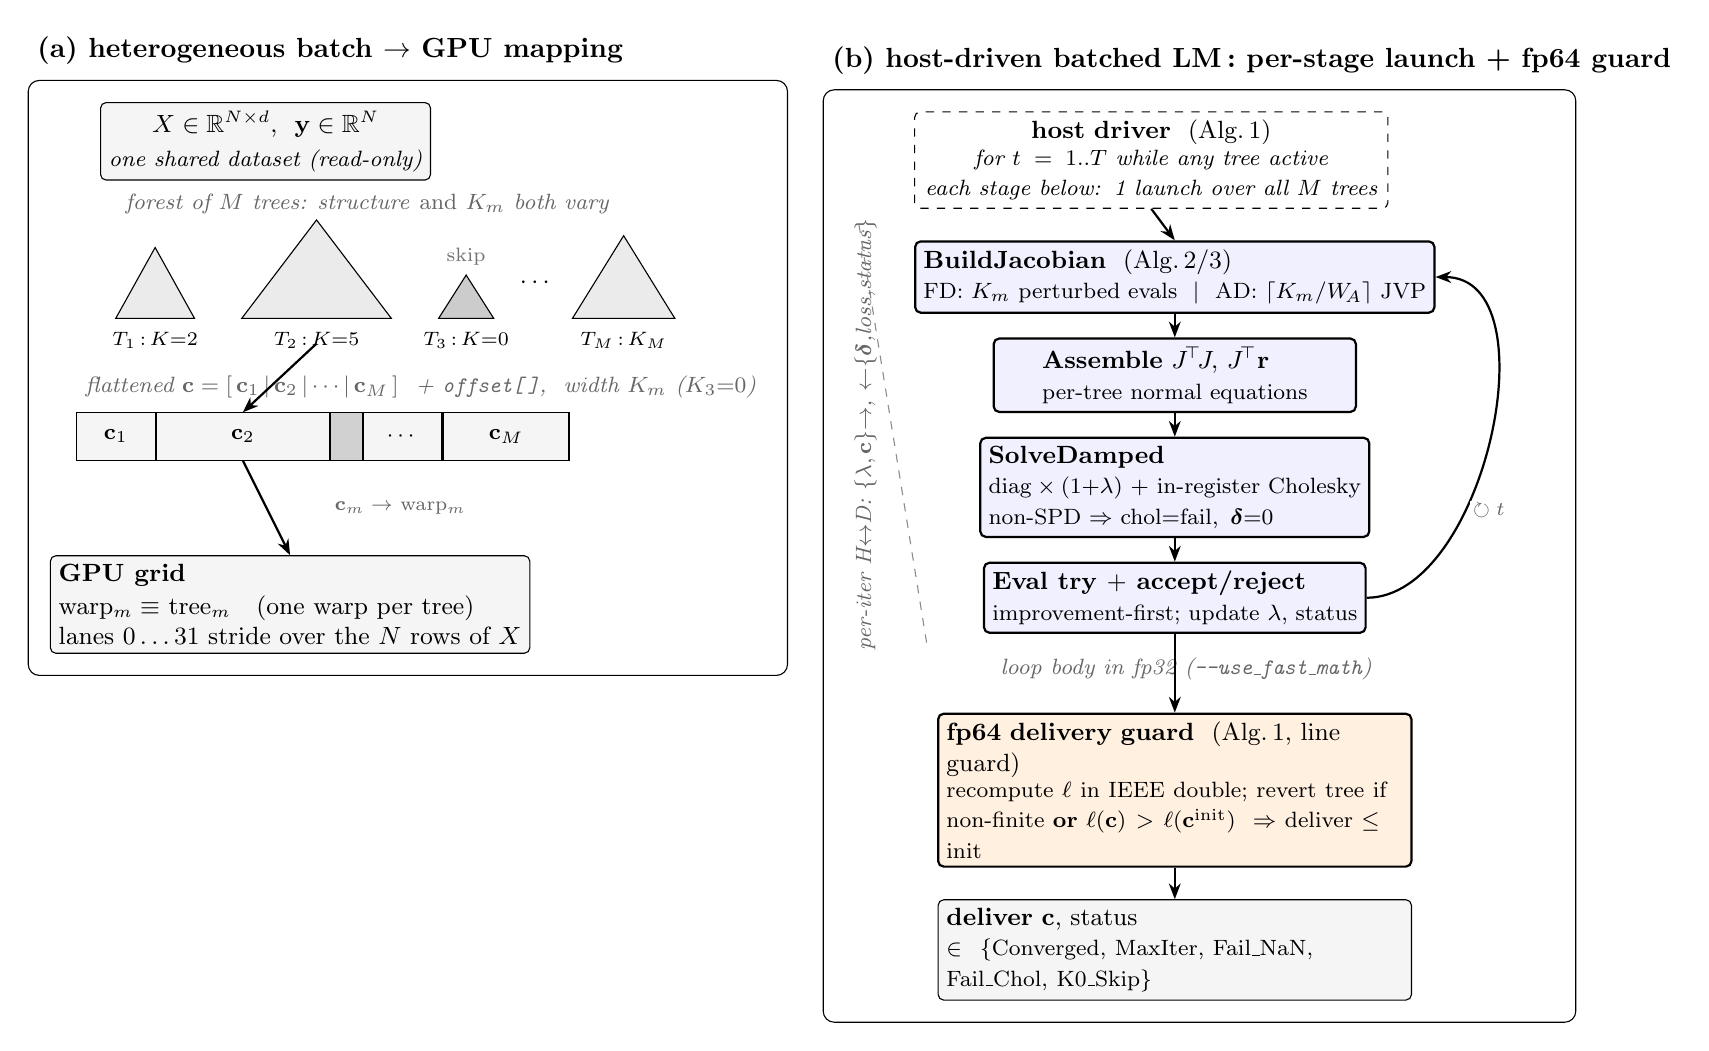
\begin{tikzpicture}[
  font=\small,
  >={Stealth[length=2mm]},
  box/.style   ={rounded corners=2pt, draw, align=center, inner sep=3pt},
  data/.style  ={box, fill=black!4},
  kern/.style  ={box, fill=blue!6, thick, minimum width=46mm, align=left},
  guard/.style ={box, fill=orange!12, thick, align=left},
  hostb/.style ={box, dashed, fill=none},
  slice/.style ={draw, minimum height=6mm, inner sep=2pt, font=\footnotesize},
  lbl/.style   ={font=\footnotesize\itshape, text=black!60},
  tag/.style   ={font=\scriptsize, fill=white, inner sep=1pt},
  fl/.style    ={->, thick},
]

% =====================================================================
% PANEL (a)  --  heterogeneous batch  ->  GPU mapping + memory layout
% =====================================================================
\begin{scope}[local bounding box=panelA]

% -- shared data --
\node[data] (data) {$X\in\mathbb{R}^{N\times d}$,\ \ $\mathbf{y}\in\mathbb{R}^{N}$\\[1pt]
  \footnotesize\itshape one shared dataset (read-only)};

% -- heterogeneous forest: triangles of different sizes = different structure --
% T1 (K=2, small), T2 (K=5, big), T3 (K=0, skip), ..., TM
\coordinate (forestO) at ($(data.south west)+(0.2,-1.75)$);
\begin{scope}[shift={(forestO)}]
  % T1 small
  \draw[fill=black!8] (0,0) -- (0.5,0.9) -- (1.0,0) -- cycle;
  \node[font=\scriptsize] at (0.5,-0.28) {$T_1$\,:\,$K{=}2$};
  % T2 large
  \draw[fill=black!8] (1.6,0) -- (2.55,1.25) -- (3.5,0) -- cycle;
  \node[font=\scriptsize] at (2.55,-0.28) {$T_2$\,:\,$K{=}5$};
  % T3 K=0 (hatched -> skipped)
  \draw[fill=black!20] (4.1,0) -- (4.45,0.55) -- (4.8,0) -- cycle;
  \node[font=\scriptsize] at (4.45,-0.28) {$T_3$\,:\,$K{=}0$};
  \node[font=\scriptsize, text=black!55] at (4.45,0.78) {skip};
  % dots + TM
  \node at (5.35,0.45) {$\cdots$};
  \draw[fill=black!8] (5.8,0) -- (6.45,1.05) -- (7.1,0) -- cycle;
  \node[font=\scriptsize] at (6.45,-0.28) {$T_M$\,:\,$K_M$};
\end{scope}
\node[lbl, anchor=west] at ($(forestO)+(0,1.45)$)
  {forest of $M$ trees: structure \emph{and} $K_m$ both vary};

% -- flattened constant array c, variable-width per-tree slices --
\node[slice, fill=black!4, minimum width=10mm] (s1) at ($(forestO)+(0.0,-1.5)$) {$\mathbf{c}_1$};
\node[slice, fill=black!4, minimum width=22mm, right=0pt of s1] (s2) {$\mathbf{c}_2$};
\node[slice, fill=black!18, minimum width=4mm, right=0pt of s2] (s3) {};
\node[slice, fill=black!4, minimum width=10mm, right=0pt of s3] (sd) {$\cdots$};
\node[slice, fill=black!4, minimum width=16mm, right=0pt of sd] (sM) {$\mathbf{c}_M$};
\node[lbl, anchor=west] at ($(s1.north west)+(0,0.32)$)
  {flattened $\mathbf{c}=[\,\mathbf{c}_1\,|\,\mathbf{c}_2\,|\cdots|\,\mathbf{c}_M\,]$\ \ +\ \texttt{offset[\,]},\ \ width $K_m$ ($K_3{=}0$)};

% -- GPU execution mapping --
\node[data, below=12mm of s2.south, xshift=6mm, align=left] (gpu)
  {\textbf{GPU grid}\\[1pt]
   warp$_m \equiv$ tree$_m$\quad(one warp per tree)\\
   lanes $0\ldots31$ stride over the $N$ rows of $X$};

\draw[fl] ($(forestO)+(2.55,-0.32)$) -- (s2.north);   % T2 -> its c-slice
\draw[fl] (s2.south) -- (gpu.north);
\node[tag, text=black!60] at ($(s2.south)!0.5!(gpu.north)+(1.7,0)$) {$\mathbf{c}_m \to$ warp$_m$};

\end{scope}

% panel (a) frame + title
\begin{scope}[on background layer]
  \node[draw, rounded corners, inner sep=8pt, fit=(panelA)] (frameA) {};
\end{scope}
\node[anchor=south west, font=\bfseries] at ([yshift=2pt]frameA.north west)
  {(a) heterogeneous batch $\to$ GPU mapping};

% =====================================================================
% PANEL (b)  --  host-driven batched LM: per-stage single launch, fp64 guard
% =====================================================================
\begin{scope}[local bounding box=panelB, shift={($(frameA.north east)+(1.6,0)$)}]

% host loop header
\node[hostb, anchor=north west, text width=58mm] (hostloop) at (0,-0.4)
  {\textbf{host driver}\ \ (Alg.\,1)\\
   \footnotesize\itshape for $t=1..T$ while any tree active\\
   \footnotesize each stage below: 1 launch over all $M$ trees};

% per-iteration device launches (each: 1 launch, all M trees, warp-per-tree)
\node[kern, below=4mm of hostloop.south west, anchor=north west] (k1)
  {\textbf{BuildJacobian}\ \ (Alg.\,2/3)\\
   \footnotesize FD: $K_m$ perturbed evals\ \ $|$\ \ AD: $\lceil K_m/W_{\!A}\rceil$ JVP};
\node[kern, below=3mm of k1] (k2)
  {\textbf{Assemble} $J^{\!\top}\!J,\,J^{\!\top}\mathbf{r}$\\
   \footnotesize per-tree normal equations};
\node[kern, below=3mm of k2] (k3)
  {\textbf{SolveDamped}\\
   \footnotesize $\mathrm{diag}\times(1{+}\lambda)$ + in-register Cholesky\\
   \footnotesize non-SPD $\Rightarrow$ $\mathrm{chol{=}fail},\ \boldsymbol\delta{=}0$};
\node[kern, below=3mm of k3] (k4)
  {\textbf{Eval try $+$ accept/reject}\\
   \footnotesize improvement-first; update $\lambda$, status};

% loop arrows
\draw[fl] (hostloop.south) -- (k1.north);
\draw[fl] (k1) -- (k2);
\draw[fl] (k2) -- (k3);
\draw[fl] (k3) -- (k4);
% loop-back
\draw[fl] (k4.east) .. controls ($(k4.east)+(1.5,0)$) and ($(k1.east)+(1.5,0)$) .. (k1.east);
\node[tag, text=black!60] at ($(k4.east)+(1.55,1.1)$) {$\circlearrowright t$};

% H<->D boundary (per-iter host round-trip; ~2-5% of runtime, not the bottleneck)
\node[lbl, rotate=90, anchor=south] at ($(k1.west)+(-0.35,-2.0)$)
  {per-iter H$\leftrightarrow$D: \{$\lambda,\mathbf{c}$\}$\to$, $\leftarrow$\{$\boldsymbol\delta$,loss,status\}};
\draw[dashed, black!45] ($(k1.north west)+(-0.7,0.2)$) -- ($(k4.south west)+(-0.7,-0.2)$);

% fp32 band label
\node[lbl, anchor=west] at ($(k4.south west)+(0.1,-0.45)$) {loop body in fp32 (\texttt{--use\_fast\_math})};

% fp64 delivery guard
\node[guard, below=10mm of k4, text width=58mm] (guard)
  {\textbf{fp64 delivery guard}\ \ (Alg.\,1, line guard)\\
   \footnotesize recompute $\ell$ in IEEE double; revert tree if\\
   \footnotesize non-finite \textbf{or} $\ell(\mathbf{c}) > \ell(\mathbf{c}^{\mathrm{init}})$\ \ $\Rightarrow$ deliver $\le$ init};
\draw[fl] (k4.south) -- (guard.north);

% output
\node[data, below=4mm of guard, text width=58mm, align=left] (out)
  {\textbf{deliver} $\mathbf{c}$, status\\
   \footnotesize $\in\{$Converged, MaxIter, Fail\_NaN, Fail\_Chol, K0\_Skip$\}$};
\draw[fl] (guard.south) -- (out.north);

\end{scope}

% fp64 band behind guard+out
\begin{scope}[on background layer]
  \node[draw, rounded corners, inner sep=8pt, fit=(panelB)] (frameB) {};
\end{scope}
\node[anchor=south west, font=\bfseries] at ([yshift=2pt]frameB.north west)
  {(b) host-driven batched LM\,: per-stage launch + fp64 guard};

\end{tikzpicture}
\end{document}
